\subsection{Thread, warp, block, grid, SM}
\begin{frame}[fragile]
  \frametitle{GPU hardware: thread, warp, block, grid, SM}
\begin{itemize}
\item GPU consists of several {\color{mycolordef}Streaming Multiprocessors (SMs)}
\item Each SM can run several thousand GPU {\color{mycolordef}threads} in parallel
\item For example, V100 has 80 SMs, K80 has 13 SMs. Each SM in those can run up to 2048 threads. Therefore up to 163840 threads can run in parallel in V100 and up to 26624 threads in K80.
\item GPU cores have much simpler logic than CPU core: do not do branch prediction, less caching
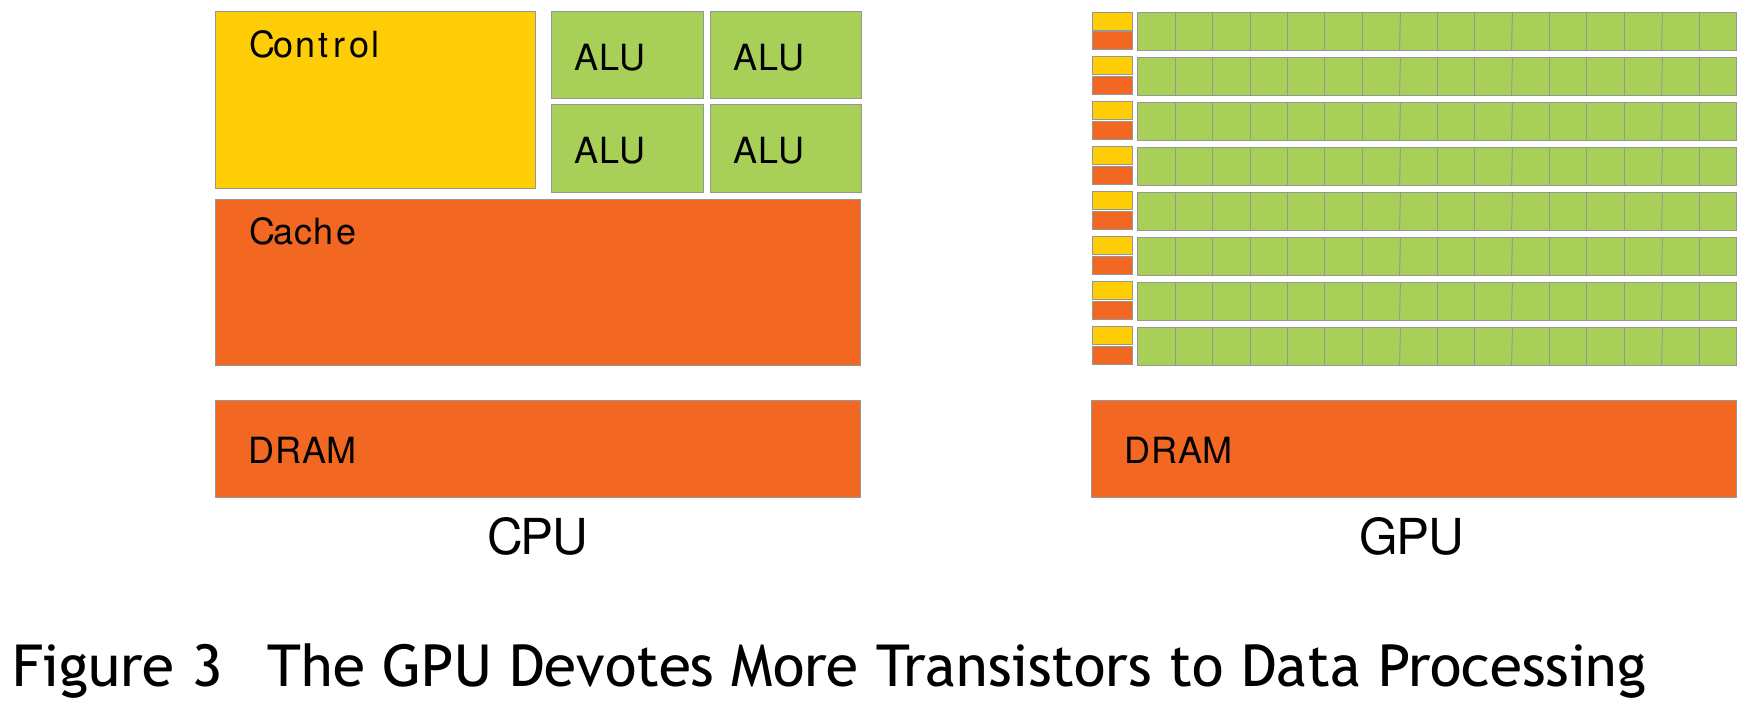
\includegraphics[width=8.5cm]{graphs/gpu_vs_cpu.png}
\end{itemize}
\end{frame}


\begin{frame}[fragile]
\begin{itemize}
\item Each GPU core is a few times slower than CPU core. For example, V100's clock frequency is 1.530 GHz, K80's - 0.824 GHz, while typical CPU clock frequencies today are around 2.5 - 3.0 GHz.
\item The threads in a job are grouped into a {\color{mycolordef}grid of blocks}
\item Each block can have up to 1024 threads
\item Blocks are scheduled to run on SMs in no particular order, in parallel  or sequentially, on the same SM or on different SMs
\item The whole block runs on one SM
\item Inside a block, threads are grouped into {\color{mycolordef}warps}
\item In a warp, there are 32 threads
\item Hardware executes each warp as a single entity
\item It is best if threads in a warp do not diverge but do the same instruction at each step
\item In case of a thread divergence in a warp due to {\color{mycolorcode}\verb|if|} statements or different lengths of loops, the divergent parts are executed sequentially
\item This architecture of GPU is called {\color{mycolordef}SIMT - Single Instruction Multiple Threads}
\end{itemize}
\end{frame}

\begin{frame}[fragile]
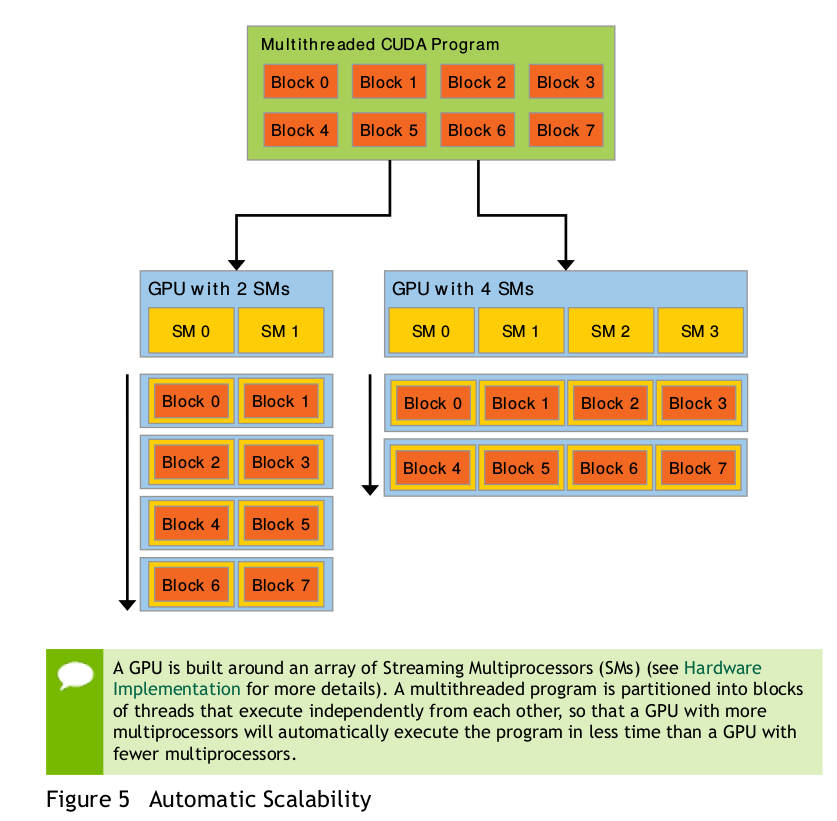
\includegraphics[width=9.0cm]{graphs/blocks_per_sm.png}
\end{frame}

\begin{frame}
\begin{columns}
\begin{column}{0.55\textwidth}
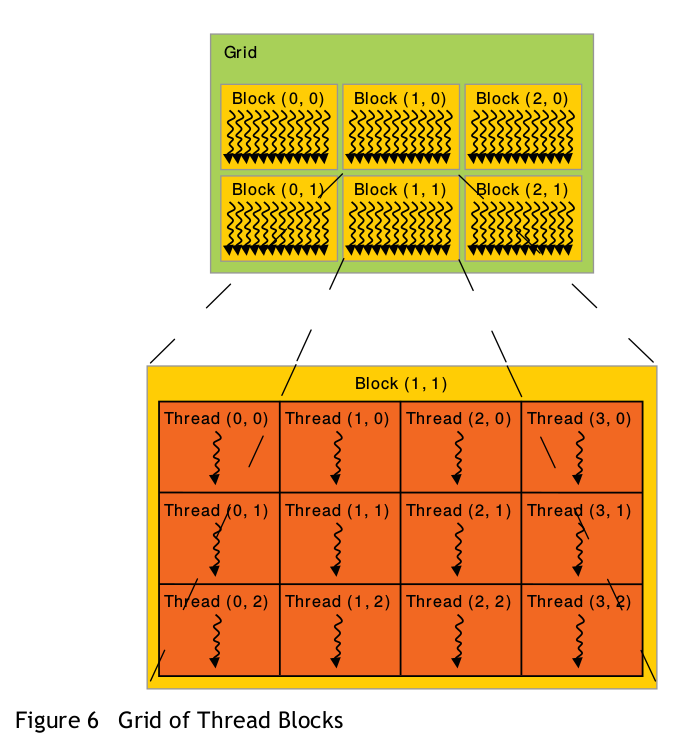
\includegraphics[width=6.5cm]{graphs/grid_of_blocks.png}
\end{column}
\begin{column}{0.45\textwidth}
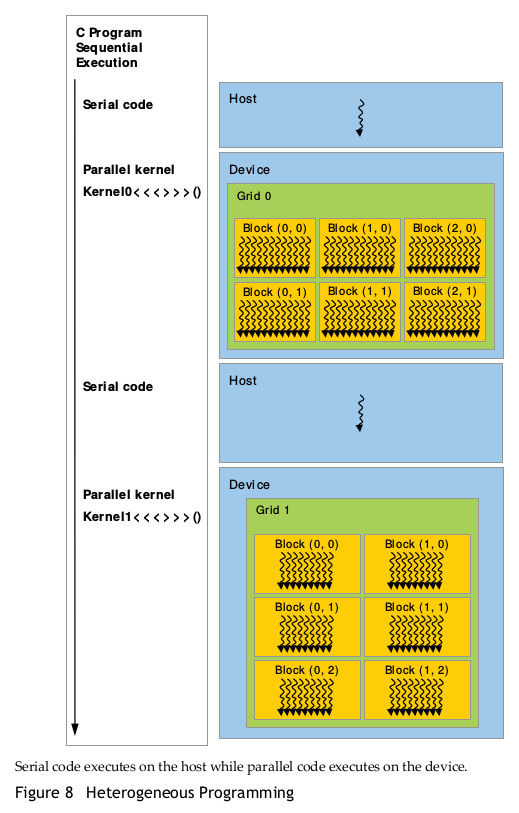
\includegraphics[width=5.5cm]{graphs/heterogeneous.png}
\end{column}
\end{columns}
\end{frame}



